% This is the Pipeline Simulation Interest Group annual meeting paper template.
% Version 1.1
%
% Notes:
% 1) please read all comments throughout the latex file
% 2) if you are having trouble with something latex related, google is your friend
% 3) last resort: email PSIG Board memmber Cody Allen: allen_cody_w@solarturbines
%
% Good luck - we look forward to your paper
%%%%%%%%%%%%%%%%%%%%%%%%%%%%%%%%%%%%%%%%%%%%%%%%%%%%%%%%%%%%%%%%%%%%%%%%%%%%%%%
%% preamble
\documentclass{psig_required_latex_files/psig}
%%%%%%%%%%%%%%%%%%%%%%%%%%%%%%%%%%%%%%%%%%%%%%%%%%%%%%%%%%%%%%%%%%%%%%%%%%%%%%%
\begin{document}
%------------------------------------------------------------------------------
% Paper number provided by PSIG
\papernumber{PSIG XXXX}
%------------------------------------------------------------------------------
% Presentation date provided by PSIG using ISO8601 date format
\presdate{2024-05-XX}
%------------------------------------------------------------------------------
% Paper title
\title{Example Title: PSIG Paper Template}
% Paper header title (used to shorten main title)
% this is optional and you can comment this out
\headertitle{PSIG Paper Template}

%------------------------------------------------------------------------------
% Author list with single corresponding author
% numbers correspond to affiliated institutions
% Notes
% make sure to follow the patterns:
%      \au{name}~\add{address_number}{\corr},~
%      \au{name}~\add{address_number}{},~
%      \au{name}~\add{address_number}{}
%
%      \au{name}~\add{address_number}{},~
%      \au{name}~\add{address_number}{\corr},~
%      \au{name}~\add{address_number}{}
%
% use \corr in the second argument of \add for the corresponding author (can be any)
% leave off the comma and ~ for the final author
%
% In the case of a single author, use:
%	  \au{name}~\add{address_number}{\corr}
%-------------------------------------------------------------------------------
\author{
\au{First Author}~\add{1}{},~
\au{Second Author}~\add{2}{\corr},~
\au{Third Author}~\add{2}{}
%\au{Fourth Author}~\add{1}{} 
}
% Addresses of authors
\address{
\add{1}{Address number one, Somewhere, Earth};
\add{2}{Address number two, SomwhereElse, Mars}
% Email of corresponding author
\email{myemail@mydomain.com}
}
%------------------------------------------------------------------------------
\maketitle
\checkheadertitle
\begin{copyrightsec} % this adds in the copyright - do not remove
\end{copyrightsec}
%%%%%%%%%%%%%%%%%%%%%%%%%%%%%%%%%%%%%%%%%%%%%%%%%%%%%%%%%%%%%%%%%%%%%%%%%%%%%%%
% start your paper below
%%%%%%%%%%%%%%%%%%%%%%%%%%%%%%%%%%%%%%%%%%%%%%%%%%%%%%%%%%%%%%%%%%%%%%%%%%%%%%%

\begin{abstract}
\lipsum[2]
\end{abstract}
 
%%%%%%%%%%%%%%%%%%%%%%%%%%%%%%%%%%%%%%%%%%%%%%%%%%%%%%%%%%%%%%%%%%%%%%%%%%%%%%%

\section{Introduction and Background}\label{sec:introd}

{\Large This is the \textcolor{orange}{PSIG \LaTeX{}} template!  }

Below we have used a mix of Lorem Ipsum gibberish text for filler along with some excerpts from a book to show how the template can be used to publish your papers!

%%%%%%%%%%%%%%%%%%%%%%%%%%%%%%%%%%%%%%%%%%%%%%%%%%%%%%%%%%%%%%%%%%%%%%%%%%%%%%%

\section{Approach}

Some filler text to show how these look next to each other.  A little bit more here and we have it.

\begin{theorem}\label{thm:thm1}
This is your awesome theorem.
\end{theorem}
\begin{proof}
This is your awesome proof. 
\end{proof}
And this leads to the following result that does not even require proof,
\begin{corollary}\label{coro:basic}
This is your corollary.
\end{corollary}

And  Theorem \ref{thm:thm1} is illustrated in Figure \ref{fig:fig1} while  Corollary \ref{coro:basic} is self-explanatory.  We can also peek ahead at the results in Table \ref{tab:tab1}.

%%%%%%%%%%%%%%%%%%%%%%%%%%%%%%%%%%%%%%%%%%%%%%%%%%%%%%%%%%%%%%%%%%%%%%%%%%%%%%%

\section{Analysis}\label{sec2}

\lipsum[6-7]

\begin{figure}
\centering{
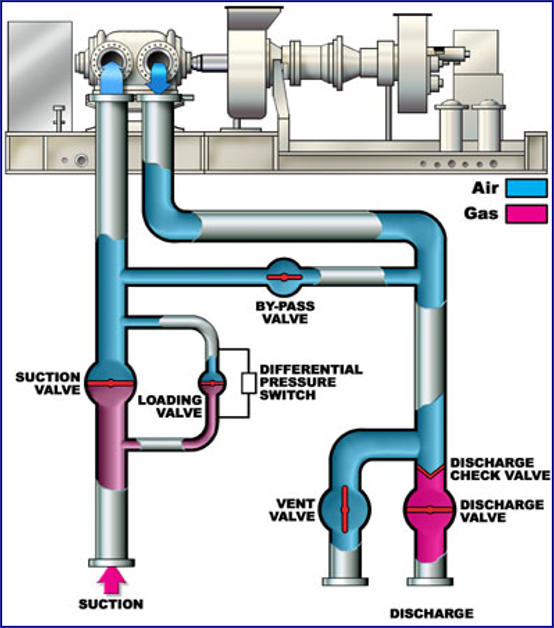
\includegraphics[width=5cm]{figs/comp_piping_and_valves.png}}
\caption{Sample figure.
%\figfooter{a}{Subfigure 1}
}\label{fig:fig1}
\end{figure}

\begin{table}
{\renewcommand{\arraystretch}{1.3}
\caption{Table of Constant Values}\label{table:1}
  \begin{center}
  \begin{tabular}{| c | c | c | c |}
    \hline
    \textbf{Measurement} & \textbf{Symbol} & \textbf{Unit} & \textbf{Value} \\ \hline
    Pressure & $P$ & $Pa$ & 101325 \\ \hline
    Temperature & $T$ & $K$ & 288 \\ \hline
    Universal Gas Constant & $R$ & $\frac{N\cdot m}{mol \cdot K}$ & 8.314 \\ \hline
    Number of Moles & $N$ & None & 1 \\ \hline
    Volume & $V$ & $m^3$ & 0.0235 \\
    \hline
  \end{tabular}
  \end{center}
}
\end{table}

\lipsum[11]

\begin{table}
\processtable{Example table of results\label{tab:tab1}}
{\begin{tabular*}{20pc}{@{\extracolsep{\fill}}lll@{}}\toprule
Column  &Column  & Column heading \\
heading  &heading two &  three \\
\midrule
Row 1a  &Row 1b  &Row 1c \\
Row 2a  &Row 2b  &Row 2c \\
Row 3a  &Row 3b  & Row 3c \\
Row 4a  &Row 4b  &Row 4c \\
Row 5a  &Row 5b  &Row 5c \\
Row 6a  & Row 6b  & Row 6c \\
\botrule
\end{tabular*}}{}
\end{table}

%------------------------------------------------------------------------------
\subsection{The Subsection}

Here is a subsection with a unordered bullet list:

\begin{itemize}
\item list item 1
\item list item 2
\item etc.
\end{itemize}

\subsubsection{And The Subsubsection without numbers}

Here is a subsubsection with an ordered bullet list:

\begin{enumerate}
\item list item 1
\item list item 2
\item etc.
\end{enumerate}



%%%%%%%%%%%%%%%%%%%%%%%%%%%%%%%%%%%%%%%%%%%%%%%%%%%%%%%%%%%%%%%%%%%%%%%%%%%%%%%

\section{Results}
The general pipe flow equation is given in \cite[Chapter 2]{GPH} as equation (2.2), shown below:
 
\begin{align}
Q_B  
&= k_f \left(\frac{T_b}{P_b} \right)\left(\frac{P_1^2 - P_2^2}{G T_f L Z f} \right)^{0.5}D^{2.5} \enskip [scfd].  \label{eq:pipe}
\end{align}


This equation is equivalent to the standard compressible flow equation for gas pipelines provided in \cite[Chapter 1]{crane1980flow} as equation 1-7a.  The Crane equation can be sourced at least to Shapiro \cite[Chapter 6]{shapiro1953dynamics} as equation (6.42).  Below we provide an account of these equations, their equivalence, and the source of their numeric values.


\begin{lemma}
Equation (1-7) of \cite{crane1980flow} can be derived from equation (6.42) of \cite{shapiro1953dynamics}
\end{lemma}
\begin{proof}
Equation (6.42) is given as
\begin{align}\label{eq:sh1}
4f\frac{L}{D} = \frac{1 - \left(\frac{p_2}{p_1} \right)^2}{kM_1^2} - \ln\left(\frac{p_1}{p_2} \right)^2.
\end{align}
Note that each term is non-dimensional.  Therefore, we may choose any absolute units we would like but momentarily hold off.  Note that $f_D = 4f$ where $f_D$ is the \emph{Darcy-Weisbach} friction factor and $f$ is sometimes referred to as the \emph{Fanning} friction factor.  By definition in Shapiro, $f = 2\tau_w / (\rho V^2)$ whereas, $f_D = 8 \tau_w/(\rho V^2)$ as given in \cite[Chapter 9]{FFM}.  Therefore, substituting in $f_D$ into \ref{eq:sh1}, we have,
\begin{align}\label{eq:sh2}
kM_1^2 = \frac{1}{f_D\frac{L}{D} + \ln\left(\frac{p_1}{p_2} \right)^2}\left(1 - \left(\frac{p_2}{p_1} \right)\right)^2
\end{align}
After some algebra and recalling that the \emph{Mach} number is $M = V/c = V/\sqrt{k R T}$, where $c$ is the speed of sound, substituting we have,
\begin{align}\label{eq:sh3}
V_1^2 &= \frac{(R T_1/p_1)}{f_D\frac{L}{D} + 2\ln\left(\frac{p_1}{p_2} \right)} \left(\frac{p_1^2 - p_2^2}{p_1} \right) \\
&= \frac{1/\rho_1}{f_D\frac{L}{D} + 2\ln\left(\frac{p_1}{p_2} \right)} \left(\frac{p_1^2 - p_2^2}{p_1} \right)
\end{align}
Define $w$ as mass flow so that $w=\rho A V$.  Define the specific volume as $\bar V = 1/\rho$.  Then, multiply both sides of \eqref{eq:sh3} by $(\rho_1 A)^2$, where $A$ is the cross sectional area,
\begin{align}\label{eq:sh4}
(\rho_1 A)^2 V_1^2 = w^2 &= \frac{A^2}{\bar V_1 \left(f_D\frac{L}{D} + 2\ln\left(\frac{p_1}{p_2} \right)\right)} \left(\frac{p_1^2 - p_2^2}{p_1} \right)
\end{align}
Now we shall establish the physical units as those used in the Crane equation.  Let pressures be given in PSIA, lengths be given in feet, density be given in lbm/ft$^3$ and mass flow in lbm/s.  In the following equation, we will put physical units in brackets. Consider the units of \eqref{eq:sh4}:
\begin{align}\label{eq:sh5}
w^2 &\enskip \left[\frac{lbm}{s}\right]^2 \\
&= \frac{A^2 \enskip [ft^2]^2 \left(\frac{p_1^2 \enskip [lbf/in^2]^2 - p_2^2 \enskip [lbf/in^2]^2}{p_1 \enskip [lbf/in^2]} \right)}{\bar V_1 \enskip [ft^3/lbm] \left(f_D\frac{L \enskip [ft]}{D \enskip [ft]} + 2\ln\left(\frac{p_1 \enskip [lbf/in^2]}{p_2\enskip [lbf/in^2]} \right)\right)} \\
&= \frac{A^2 \enskip \left(\frac{p_1^2  - p_2^2}{p_1 } \right)}{\bar V_1 \left(f_D\frac{L}{D } + 2\ln\left(\frac{p_1 }{p_2} \right)\right)}\left[\frac{lbm \cdot lbf \cdot ft}{in^2}\right] \\
&= \frac{144  A^2  \left(\frac{p_1^2  - p_2^2}{p_1 } \right)}{\bar V_1 \left(f_D\frac{L}{D } + 2\ln\left(\frac{p_1 }{p_2} \right)\right)}\left[\frac{lbm \cdot lbf}{ft}\right]
\end{align}
Finally, recalling that $1 \enskip [lbf] = 32.174 \enskip [lbm \cdot ft/s^2] = g \enskip [lbm \cdot ft/s^2]$, we have,
\begin{align}\label{eq:c6}
w^2 \enskip \left[\frac{lbm}{s}\right]^2 &= \frac{ 144g A^2  \left(\frac{p_1^2  - p_2^2}{p_1 } \right)}{\bar V_1 \left(f_D\frac{L}{D } + 2\ln\left(\frac{p_1 }{p_2} \right)\right)}\left[\frac{lbm}{s}\right]^2
\end{align}

Equation \ref{eq:c6} is precisely equation 1-6 in \cite{crane1980flow}.  Adding the assumption that acceleration can be neglected drops the term $2\ln(p1/p2)$:
\begin{align}\label{eq:c7}
w^2  &= \frac{ 144g D A^2  }{\bar V_1 f_D L }\left(\frac{p_1^2  - p_2^2}{p_1 } \right)
\end{align}
and we have arrived at equation 1-7 as desired.
\end{proof}

Showing the equivalence of the general flow equation expressed as a mass flow compared with volumetric flow is hardly a lemma, however, we will state it here and prove it for the sake of completeness, as we will end by showing that the equations found in Crane and Menon are identical.
\begin{lemma}
Equation (1-7) and (1-7a) in \cite[Chapter 1]{crane1980flow} are equivalent.
\end{lemma}
\begin{proof}
Consider \eqref{eq:c7} with mass flow $w$.  Dividing $w$ by $\rho_g$, the specific gas density, at standard conditions will provide an equation of volumetric flow at standard conditions $[ft^3/s]$.  Recall that $\rho_g = S_g \rho_a$ where $S_g$ is the specific gravity and $\rho_a$ is the density of air.  Furthermore, $R=53.3/S_g$ and for an ideal gas, $\rho = p/RT$. However, for the units specified in Crane for $\rho \enskip [lbm/ft^3]$, we must convert the pressure length scale to feet, which yields $\rho = 144p/RT$. We have, 
\begin{align}
q &= \frac{w}{\rho_g} = \sqrt{\frac{144 g D A^2 \rho_1}{f L (\rho_a S_g)^2} \frac{(p_1^2 - p_2^2)}{p_1}} \nonumber \\
&= \sqrt{\frac{144 g D A^2 \rho_1}{f L (\rho_a S_g)^2 } \frac{RT}{RT}\frac{(p_1^2 - p_2^2)}{\frac{144}{144}p_1}} \nonumber\\
&= \sqrt{\frac{144^2 g D A^2 }{\rho_a^2 f L S_g^2 (53.3/S_g)T} (p_1^2 - p_2^2)} \nonumber \\
&= \sqrt{\frac{144^2 g D A^2 }{53.3 \rho_a^2 f L S_g T} (p_1^2 - p_2^2)} \label{eq:c71}
\end{align}
Now, $A = (\pi/4)^2 D^4$, and $\rho_a = 0.0764$ at standard conditions is used in Crane \cite[Appendix B]{crane1980flow}.  Then, substituting these and $g = 32.2$ into \eqref{eq:c71} and simplifying, we have,
\begin{align}\label{eq:c72}
q &=  \sqrt{\frac{144^2 \cdot 32.2 \cdot \pi^2}{16 \cdot 53.3 \cdot (0.0767)^2}} \sqrt{\frac{D^5 }{f L S_g T} (p_1^2 - p_2^2)}
\end{align}
Finally, we must adjust the units of $L$ and $D$.  $L \enskip [ft] = 5280 L_m \enskip [miles]$ and $D \enskip [ft] = 12 d \enskip [in]$.  Therefore, \eqref{eq:c72} becomes
\begin{align}
q &=  \sqrt{\frac{144^2 \cdot 32.2 \cdot \pi^2}{16 \cdot 53.3 \cdot (0.0767)^2}} \sqrt{\frac{(\frac{12d}{12})^5 }{f \frac{5280 L_m}{5280} S_g T} (p_1^2 - p_2^2)} \nonumber \\
&=  \sqrt{\frac{144^2 \cdot 32.2 \cdot \pi^2}{16 \cdot 53.3 \cdot (0.0767)^2 \cdot 5280 \cdot 12^5 }} \sqrt{\frac{d^5 }{f L_m S_g T} (p_1^2 - p_2^2)} \label{eq:c73}\\
&\approx 0.0317 \sqrt{\frac{d^5 }{f L_m S_g T} (p_1^2 - p_2^2)}
\end{align}
Finally, to change the flow units from $[ft^3/s]$ to $[ft^3/hr]$ we multiply by 3600:
\begin{align}\label{eq:c74}
q_h = 114.2 \sqrt{\frac{(p_1^2 - p_2^2) d^5 }{f L_m T S_g } }
\end{align}
which yields equation (1-7a) as desired.
\end{proof}


\begin{theorem}
Equation (1-7a) of \cite[Chapter 1]{crane1980flow} and equation (2.2) of \cite{GPH} are equivalent.
\end{theorem}
\begin{proof}
Since $T_B = 520 \enskip [^\circ R]$ and $P_B = 14.7 \enskip [psia]$, we have have
\begin{align*}
\frac{77.54}{24}\cdot\frac{520}{14.7} \approx 114.2
\end{align*}
where the division by $24$ is to convert from per day to per hour.  The remaining piece is bringing in the compressibility factor $Z$.  Crane assumes ideal gas whereas Menon uses real gas.  The correction factor alters the ideal gas equation from $\rho = P/RT$ to $\rho = P/ZRT$.  This manifests in the second line of equations given in \eqref{eq:c71}, where instead of substituting in $1 = RT/RT$ we substitute  $1 = ZRT/ZRT$, which leaves $Z$ in the denominator.

Thus, with these substitutions, equation (2.2) of \cite[Chapter 2]{GPH} given in \eqref{eq:pipe} becomes equation (1-7a) of \cite[Chapter 1]{crane1980flow} given in \eqref{eq:c74}.  

While the above is accurate, it is not entirely satisfying. Consider \eqref{eq:c73}, where we bring back $\rho_a = P/RT$.  Note that $\rho_a = 0.0767 \enskip [lbm/ft^3] = 144 P/R_a T$ and $R_a = 53.3$:
\begin{align}
q &=  \sqrt{\frac{144^2 \cdot 32.2 \cdot \pi^2}{16 \cdot 53.3  \cdot 5280 \cdot 12^5 }} \sqrt{\frac{(p_1^2 - p_2^2) d^5 }{\rho_a^2 f L_m S_g T} } \nonumber \\
&=  \sqrt{\frac{144^2 \cdot 32.2 \cdot \pi^2}{16 \cdot 53.3  \cdot 5280 \cdot 12^5 }} \sqrt{\frac{(p_1^2 - p_2^2) d^5 }{\left(\frac{144 P_B}{R_a T_B} \right)^2 f L_m S_g T} } \nonumber\\
&=   \sqrt{\frac{ 53.3 \cdot 32.2 \cdot \pi^2}{16   \cdot 5280 \cdot 12^5 }}\left( \frac{T_B}{P_B}\right)\sqrt{\frac{(p_1^2 - p_2^2) d^5 }{ f L_m S_g T} } \nonumber\\
&\left(\approx 8.9766\times 10^{-4}\right)\left(\frac{T_B}{P_B}\right)\sqrt{\frac{(p_1^2 - p_2^2) d^5 }{ f L_m S_g T}} \label{eq:c75}
\end{align}
and since $q$ has units $[ft^3/s]$ at standard conditions, we must multiply \eqref{eq:c75} by $8.64 \times 10^4$ which gives the final result $Q \enskip [ft^3/day]$ at standard condtions:
\begin{align}
Q = 77.76\left(\frac{T_B}{P_B}\right)\sqrt{\frac{(p_1^2 - p_2^2) d^5 }{ f L_m S_g T} }
\end{align}
which is equation \eqref{eq:pipe} up to rounding.
\end{proof}


%%%%%%%%%%%%%%%%%%%%%%%%%%%%%%%%%%%%%%%%%%%%%%%%%%%%%%%%%%%%%%%%%%%%%%%%%%%%%%%
\section{Results}\label{sec3}
\lipsum[7-8]

\begin{figure*}[!b]
\centering{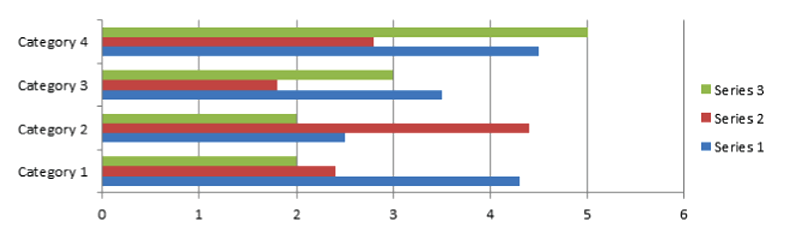
\includegraphics{figs/sample_2.eps}}
\caption{Sample graph spaning two columns and using .eps style instead of .png}\label{fig2}
\end{figure*}


%%%%%%%%%%%%%%%%%%%%%%%%%%%%%%%%%%%%%%%%%%%%%%%%%%%%%%%%%%%%%%%%%%%%%%%%%%%%%%%
\section{Conclusion}\label{sec4}
\lipsum[10]

%%%%%%%%%%%%%%%%%%%%%%%%%%%%%%%%%%%%%%%%%%%%%%%%%%%%%%%%%%%%%%%%%%%%%%%%%%%%%%%

%%%%%%%%%%%%%%%%%%%%%%%%%%%%%%%%%%%%%%%%%%%%%%%%%%%%%%%%%%%%%%%%%%%%%%%%%%%%%%%%%%%%
\section*{Acknowledgments}\label{sec11}

Acknowledgements should be placed after the conclusion and before the
references section. This is where reference to any grant numbers or
supporting bodies should be included. 


%%%%%%%%%%%%%%%%%%%%%%%%%%%%%%%%%%%%%%%%%%%%%%%%%%%%%%%%%%%%%%%%%%%%%%%%%%%%%%%
% references
\bibliographystyle{ieeetr}
\bibliography{references}
% uses a references.bib bibtex file


%%%%%%%%%%%%%%%%%%%%%%%%%%%%%%%%%%%%%%%%%%%%%%%%%%%%%%%%%%%%%%%%%%%%%%%%%%%%%%%
\section*{Appendices}\label{sec:app}

Additional material, e.g. mathematical derivations, tables and figures
larger than half a page that may interrupt the flow of your paper's argument
should form a separate Appendix section.

\begin{table*}[ht]
\caption{Example wide single-column table in a twocolumn document.}
\centering
\begin{tabular}{p{0.25\linewidth}p{0.25\linewidth}p{0.25\linewidth}}
\hline
column 1 & column 2 & column 3\\
\hline
cell 1 & cell 2 & cell 3\\
cell 1 & cell 2 & cell 3\\
\hline
\end{tabular}
\end{table*}

%%%%%%%%%%%%%%%%%%%%%%%%%%%%%%%%%%%%%%%%%%%%%%%%%%%%%%%%%%%%%%%%%%%%%%%%%%%%%%%

\section*{Author Biographies}

\textbf{Author One} - has this background.

\noindent
\textbf{Author Two} - has that background.

\noindent
\textbf{Author Three} - has another background.

%%%%%%%%%%%%%%%%%%%%%%%%%%%%%%%%%%%%%%%%%%%%%%%%%%%%%%%%%%%%%%%%%%%%%%%%%%%%%%%
\end{document}
